
\documentclass[a4paper,11pt]{article}%,twocolumn
%% packages

\usepackage{blindtext} % needed for creating dummy text passages
%\usepackage{ngerman} % needed for German default language
\usepackage{amsmath} % needed for command eqref
\usepackage{amssymb} % needed for math fonts
\usepackage[colorlinks=true,breaklinks]{hyperref} % needed for creating hyperlinks in the document, the option colorlinks=true gets rid of the awful boxes, breaklinks breaks lonkg links (list of figures), and ngerman sets everything for german as default hyperlinks language
\usepackage[hyphenbreaks]{breakurl} % ben�tigt f�r das Brechen von URLs in Literaturreferenzen, hyphenbreaks auch bei links, die �ber eine Seite gehen (mit hyphenation).
\usepackage{xcolor}
\definecolor{c1}{rgb}{0,0,1} % blue
\definecolor{c2}{rgb}{0,0.3,0.9} % light blue
\definecolor{c3}{rgb}{0.3,0,0.9} % red blue
\hypersetup{
    linkcolor={c1}, % internal links
    citecolor={c2}, % citations
    urlcolor={c3} % external links/urls
}
%\usepackage{cite} % needed for cite
\usepackage[square,authoryear]{natbib} % needed for cite and abbrvnat bibliography style
\usepackage[nottoc]{tocbibind} % needed for displaying bibliography and other in the table of contents
\usepackage{graphicx} % needed for \includegraphics 
\usepackage{longtable} % needed for long tables over pages
\usepackage{bigstrut} % needed for the command \bigstrut
\usepackage{enumerate} % needed for some options in enumerate
%\usepackage{todonotes} % needed for todos
\usepackage{makeidx} % needed for creating an index
\makeindex
\usepackage{gensymb}
\usepackage{url}
\usepackage{psfrag}
\usepackage{multirow}
\usepackage{subfigure}
%% page settings

\usepackage[top=20mm, bottom=20mm,left=15mm,right=15mm]{geometry} % needed for page border settings
\parindent=0mm % for space of first line of new text block
\sloppy % for writing with hyphenless justification (tries to)
\hyphenation{} % use hyphenation of tolerance parametershttp://www.jr-x.de/publikationen/latex/tipps/zeilenumbruch.html
\hyphenpenalty=10000
\exhyphenpenalty=10000
\usepackage{fancyhdr} % needed for head and foot options
%% my macros

%% Text fomats
\newcommand{\tbi}[1]{\textbf{\textit{#1}}}

%% Math fonts
\newcommand{\bbA}{\mathbb{A}}
\newcommand{\bbB}{\mathbb{B}}
\newcommand{\bbC}{\mathbb{C}}
\newcommand{\bbD}{\mathbb{D}}
\newcommand{\bbE}{\mathbb{E}}
\newcommand{\bbF}{\mathbb{F}}
\newcommand{\bbG}{\mathbb{G}}
\newcommand{\bbH}{\mathbb{H}}
\newcommand{\bbI}{\mathbb{I}}
\newcommand{\bbJ}{\mathbb{J}}
\newcommand{\bbK}{\mathbb{K}}
\newcommand{\bbL}{\mathbb{L}}
\newcommand{\bbM}{\mathbb{M}}
\newcommand{\bbN}{\mathbb{N}}
\newcommand{\bbO}{\mathbb{O}}
\newcommand{\bbP}{\mathbb{P}}
\newcommand{\bbQ}{\mathbb{Q}}
\newcommand{\bbR}{\mathbb{R}}
\newcommand{\bbS}{\mathbb{S}}
\newcommand{\bbT}{\mathbb{T}}
\newcommand{\bbU}{\mathbb{U}}
\newcommand{\bbV}{\mathbb{V}}
\newcommand{\bbW}{\mathbb{W}}
\newcommand{\bbX}{\mathbb{X}}
\newcommand{\bbY}{\mathbb{Y}}
\newcommand{\bbZ}{\mathbb{Z}}


% Define colors
\definecolor{codegreen}{rgb}{0,0.6,0}
\definecolor{codegray}{rgb}{0.5,0.5,0.5}
\definecolor{codepurple}{rgb}{0.58,0,0.82}
\definecolor{backcolour}{rgb}{0.95,0.95,0.92}
% Setup the listings package
\lstset{
    backgroundcolor=\color{backcolour},   
    commentstyle=\color{codegreen},
    keywordstyle=\color{magenta},
    numberstyle=\tiny\color{codegray},
    stringstyle=\color{codepurple},
    basicstyle=\footnotesize,
    breakatwhitespace=false,         
    breaklines=true,                 
    captionpos=b,                    
    keepspaces=true,                 
    numbers=left,                    
    numbersep=5pt,                  
    showspaces=false,                
    showstringspaces=false,
    showtabs=false,                  
    tabsize=2
}



\begin{document}
\begin{titlepage}
\center % Center everything on the page

%-------------------------------------------------------------------------------------
%	HEADING SECTIONS
%------------------------------------------------------------------------------------
\textbf{\large Department of Electrical and Computer Engineering}\\[0.5cm]
\textbf{\Large University of Colorado at Boulder}\\[1cm]
\textbf{\large ECEN5730 - Practical PCB design}\\[2cm]

\includegraphics[width=0.3\textwidth]{figures/cu}\\[2cm] 

	
%-------------------------------------------------------------------------------------
%	TITLE SECTION
%------------------------------------------------------------------------------------

\textbf{\Huge Board Good Layout/Bad Layout }\\[0.2cm]

\textbf{\Large Report}\\[2cm]
\vspace{1.5cm}
\begin{figure}[H]
	\centering
	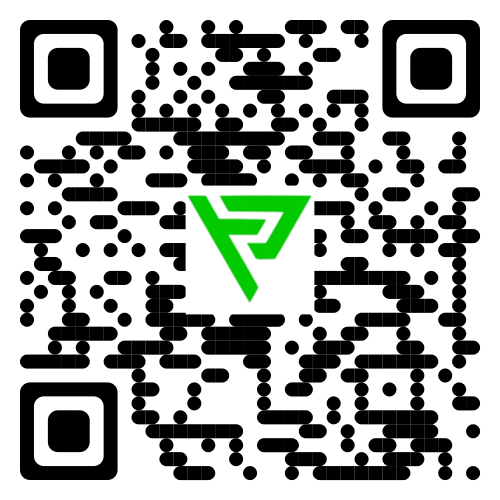
\includegraphics[scale=0.2]{figures/qr_download.png}
	\label{555_schematic}
\end{figure}\vspace{1.5cm}


%----------------------------------------------------------------------------------------
%	MEMBERS SECTION
%----------------------------------------------------------------------------------------


\vfill

\textbf{\large Submitted by}

{\large Parth Thakkar}\\[0.5cm]




%----------------------------------------------------------------------------------------
%	DATE SECTION
%----------------------------------------------------------------------------------------

\textbf{\large Submitted on}\\
\textbf{\Large \today} % Date, change the \today to a set date if you want to be precise

%----------------------------------------------------------------------------------------

\vfill % Fill the rest of the page with whitespace

\end{titlepage}

\pagebreak

\tableofcontents
\listoffigures
\listoftables
\vfill
\begin{center}
	\textbf{\textit{*PDF is clickable}}
\end{center}

\pagebreak

\section{Objective / Purpose of Lab}

\begin{itemize}
	\item DMM Measurements of 2-Wire Resistance: Understanding the basics of using a digital multimeter (DMM) to measure resistance in a simple two-wire configuration.
	4-Wire Resistance Measurements: Learning the advanced technique of four-wire (Kelvin) resistance measurement, which improves accuracy by eliminating the resistance of the measurement leads and validate their estimations against real-world values.
	\item experimentally determine the maximum current carrying capacity of electrical traces of different widths (specifically 6 mil and 20 mil wide traces) by connecting them to increasing amounts of current until they fail. This experiment aims to understand the relationship between trace width, and max current flow\\
	
	Here is the board that we have to use for trace resistance and blowing up traces
	\begin{figure}[!h]
		\centering
		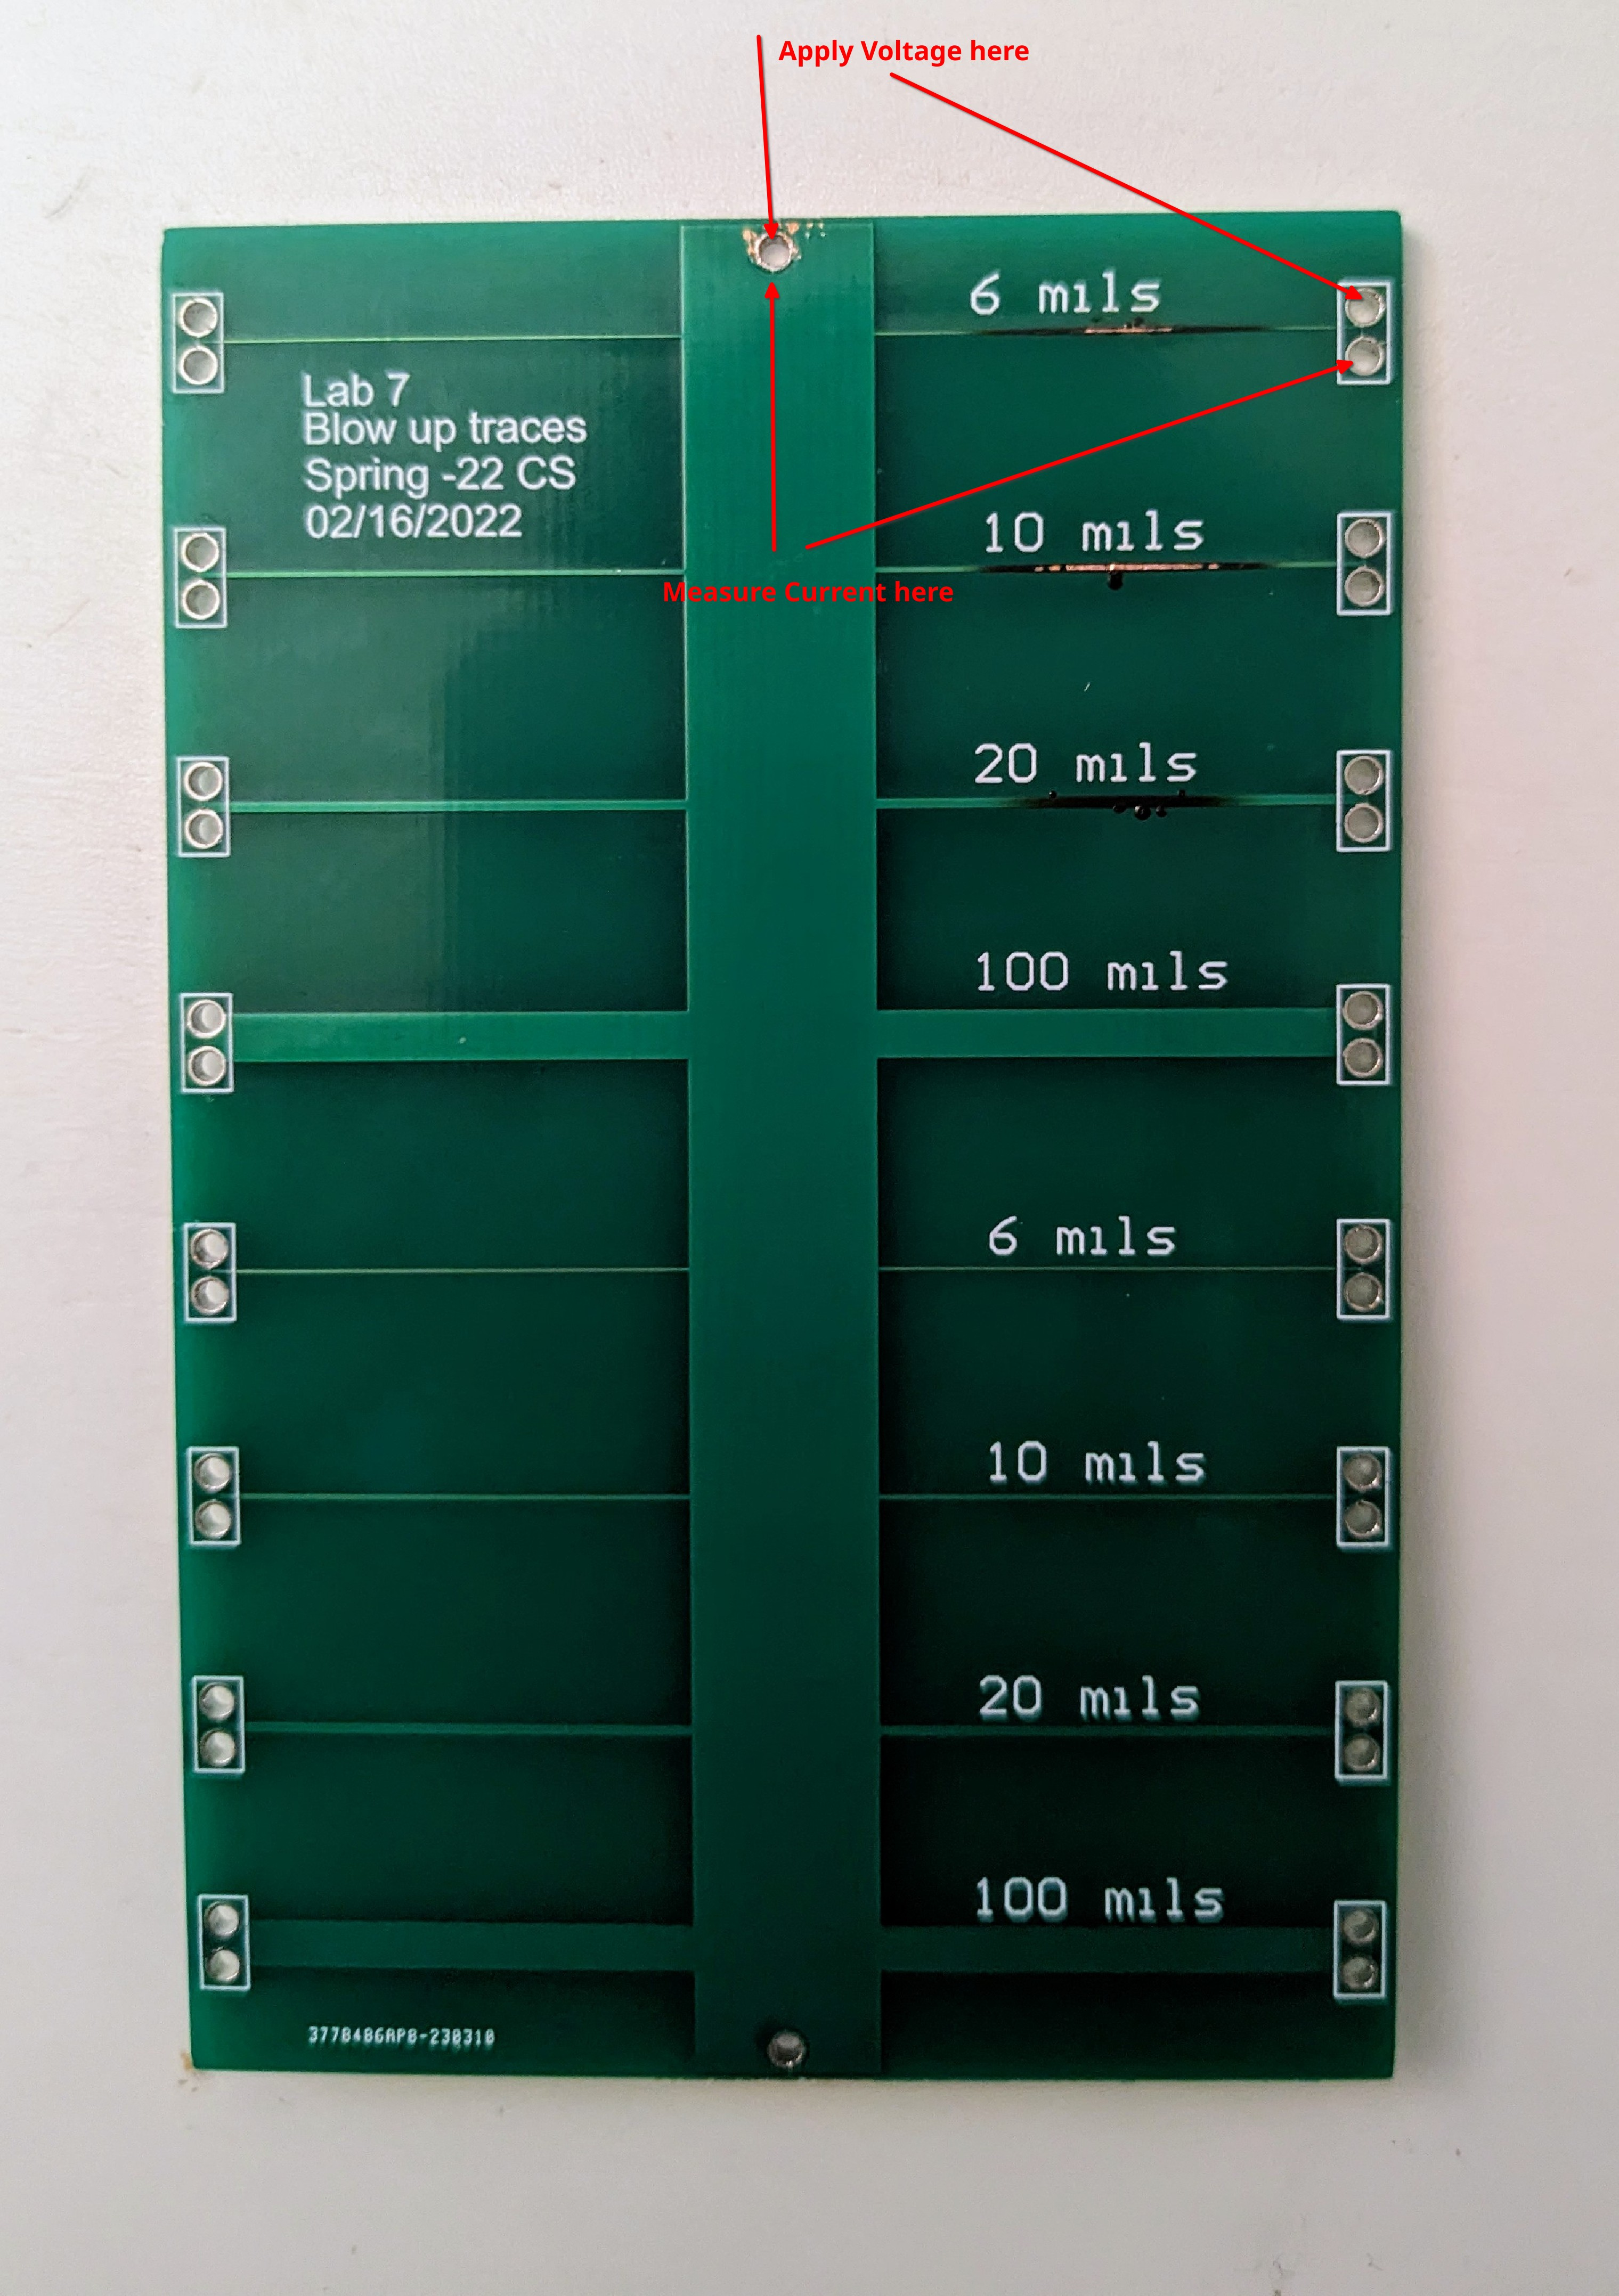
\includegraphics[scale=0.12]{figures/4wire}
		\caption{PCB}

	\end{figure}
	
\end{itemize}


\section{Component listing}


\begin{table}[H]
	\centering 
	\begin{tabular}{|c|l|}
		\hline
		&\textbf{Component Name}\\\hline
		\cr
		1&Digital Multimeter (DMM)\\
		2&Constant current and constant voltage power supply\\
3&Test PCB with various trace widths (6 mils, 10 mils, 20 mils, 100 mils) and 1-inch length\\
4&Cables and connectors for measurement (including banana cables for high current)\\
\hline\hline
	\end{tabular}
	\caption{Component list}
	\label{filterspecs}
\end{table}





\section{Explanation}

\subsection{2-Wire Method}
The 2-wire method is the simplest form of resistance measurement. In this method, two wires are used to connect the meter to the resistor being tested. The setup involves running a current through the resistor and measuring the voltage across it. The resistance is then calculated using Ohm's law (R = $\frac{V}{I}$).\\

\textbf{Limitations:}
\begin{enumerate}
	\item \textbf{Lead Resistance:} The major limitation of the 2-wire method is the inclusion of lead resistance in the measurement. The resistance of the wires used to connect the meter to the resistor adds to the total resistance being measured. This is particularly problematic when measuring very low resistances, as the lead resistance can be significant in comparison to the resistance of the device being measured.
	Accuracy: Due to the added lead resistance, the accuracy of the 2-wire method decreases for low-value resistances.
\end{enumerate}

\subsection{4-Wire (Kelvin) Method}
The 4-wire method, also known as the Kelvin method, is a more accurate technique for measuring resistance, especially useful for low resistance values. It uses four wires, two for carrying the current (source leads) and two for sensing the voltage (sense leads).

\textbf{How It Works:}
\begin{enumerate}
	\item \textbf{Current Source Leads:} These leads deliver the measurement current to the resistor. The current flows through the resistor and creates a voltage drop across it due to its resistance.
	\item \textbf{Voltage Sense Leads:} These leads are connected across the resistor, very close to the resistor terminals, to accurately measure the voltage drop. Because these leads only need to sense the voltage and do not carry the measurement current, the voltage drop across them is negligible, effectively eliminating the effect of lead resistance on the voltage measurement.
	\item Using KVL we can estimate the Resistance across the probes
\end{enumerate}


\textbf{Advantages:}

\begin{enumerate}
	\item \textbf{Accuracy:} The 4-wire method significantly improves measurement accuracy, especially for low-resistance measurements, by eliminating the influence of lead resistances on the voltage measurement.
	\item \textbf{Application:} It is widely used in precision measurements in laboratories and industrial settings, particularly for measuring the resistance of components where even a small error due to lead resistance is unacceptable.
\end{enumerate}


\textbf{Practical Considerations:}

The 4-wire method requires a more complex setup and instrumentation compared to the 2-wire method. Devices specifically designed for 4-wire resistance measurement, known as Kelvin meters or 4-wire ohmmeters, are used.
Proper connection is crucial to avoid introducing errors. The sense leads must be connected directly to the resistor terminals, bypassing any connection resistance that might be present.

\section{Procedure}

\begin{enumerate}
	\item \textbf{Analyze the Test Board:} Use the DMM to verify the connections on the test board through reverse engineering.
	\item \textbf{Resistance Measurement:}
	Measure the resistance of the 1-inch long test lines using the 2-wire method.
	\item Repeat the measurement using the 4-wire method to compare results.
\end{enumerate}





\textbf{Estimation using Saturn PCB Toolkit:}

Use the Saturn PCB Toolkit to estimate the maximum current that a 6 mil and a 20 mil wide trace can safely carry without exceeding a 40°C temperature rise.
Record these estimated values for comparison with experimental results.

for blowing up traces
Preparation for Experimental Measurement:

Set up the power supply, voltmeter, and PCB for a 4-wire measurement according to the lab manual instructions.


Incrementally increase the current through the trace while monitoring its temperature by touch and the voltage across it using the voltmeter.
Record the current values at which the trace feels noticeably warm, hot to the touch, and begins to smoke.
Observe and note the resistance changes as the trace heats up, using the 4-wire measurement method.


\section{Calculations}

\subsection{Lab 10: Resistance through 2-Wire method and 4-Wire method}
\textbf{2-Wire Method Calculations}
In the 2-wire method, you measure the total resistance by multimeter with setting probes directly on traces, the measurement includes probe resistance as well. \\

$R_{total} = R_{lead1} + R_{lead2} + R_{load}$\\
In an ideal scenario, you want to measure just 
$R_{load}$, but in the 2-wire method, the lead resistances (
$R_{lead1}$ and $R_{load}$ ) add to the total measured resistance. Without knowing the exact values of $R_{lead1}$ and $R_{load}$, it's difficult to accurately calculate using this method alone, especially for low-resistance measurements where the lead resistances may be significant relative to the load resistance.\\

\textbf{4-Wire (Kelvin) Method Calculations}
The 4-wire method separates the current path from the voltage measurement path to eliminate the effect of lead resistances on the voltage measurement. You still run a known current I through the resistor ( $R_{load}$ ), but now you measure the voltage drop directly across the resistor, not including the leads, using a separate pair of leads.
The resistance of the resistor is then calculated using the formula derived from Ohm's law:\\

$R = \frac{V}{I}$\\


In this setup:\\

I is the current flowing through the resistor, introduced through the current source leads. $V_{load}$ is the voltage drop measured across the resistor, using the voltage sense leads.Because the voltage sense leads do not carry the measurement current, their resistance does not affect the voltage drop measurement. Therefore, the calculated accurately reflects only the resistance of the resistor, free from the influence of lead resistances.



\section{Measurement}


\subsection{Lab 10: Resistance through 2-Wire method and 4-Wire method}
\begin{figure}[H]
\centering
% First image
\begin{minipage}[b]{0.45\linewidth}
	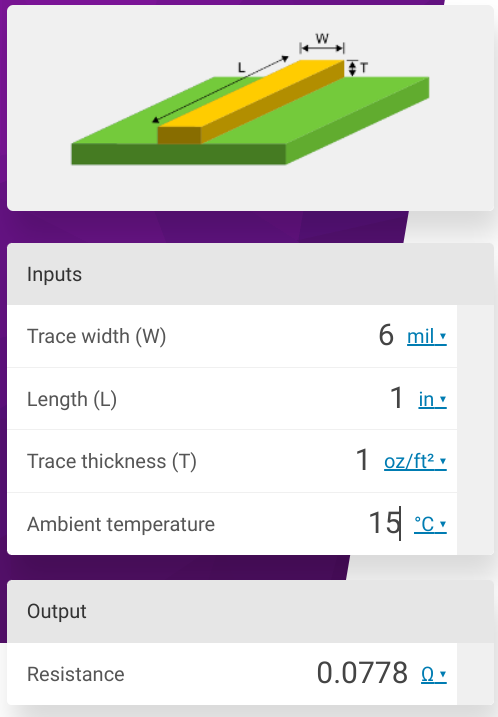
\includegraphics[scale=0.4]{figures/6}
	\caption{6mil Trace (1 inch length) }
\end{minipage}
\
% Second image
\begin{minipage}[b]{0.45\linewidth}
	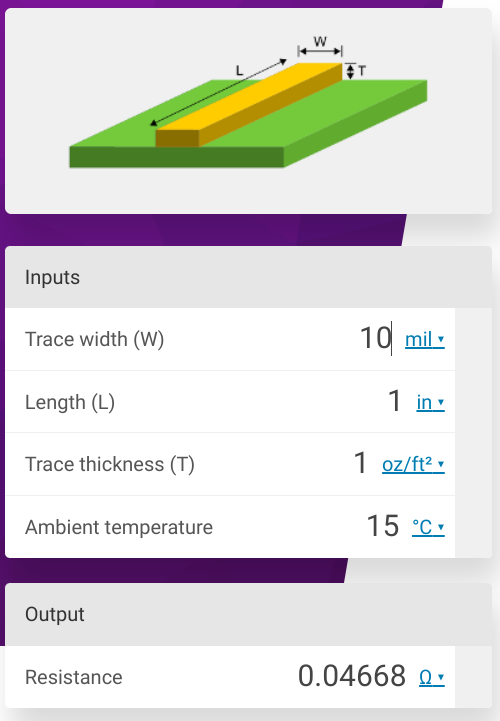
\includegraphics[scale=0.4]{figures/10}
	\caption{10mil Trace (1 inch length) }
\end{minipage}
\end{figure}\hspace{1cm}


\begin{figure}[H]
\centering
\begin{minipage}[b]{0.45\linewidth}
	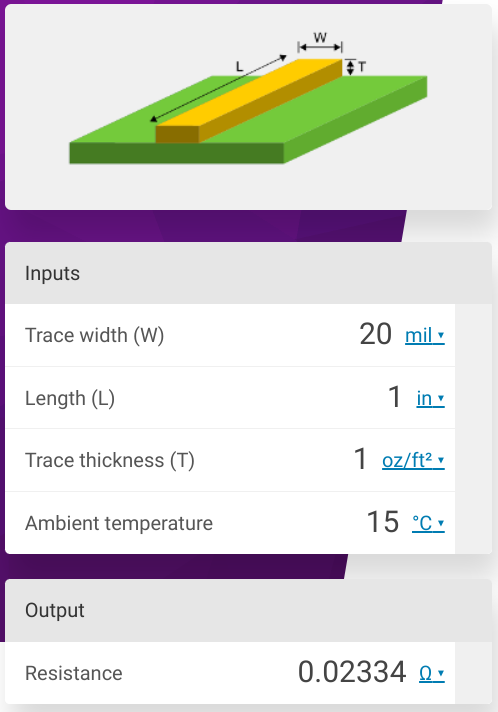
\includegraphics[scale=0.4]{figures/20}
	\caption{20mil Trace (1 inch length) }
\end{minipage}
\
\begin{minipage}[b]{0.45\linewidth}
	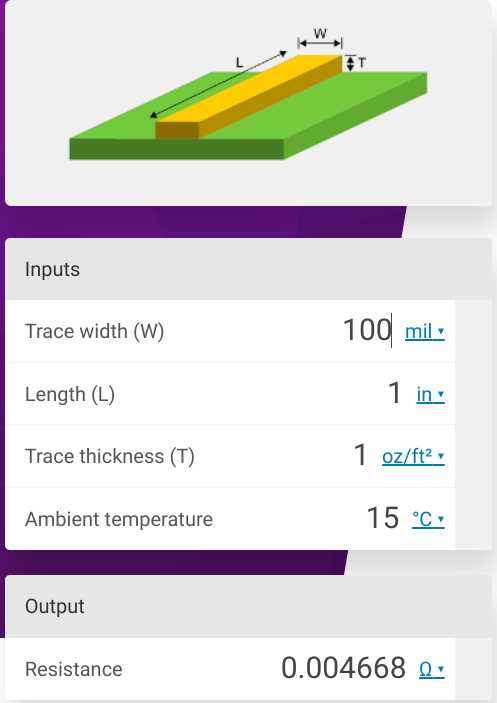
\includegraphics[scale=0.4]{figures/100}
	\caption{100mil Trace (1 inch length) }
\end{minipage}
\end{figure}


\begin{table}[H]
	\centering 
	\begin{tabular}{| l | c | c c c | c |}
		\hline
		\textbf{Trace witdth}&\textbf{R (2 Wire)}&\textbf{V}&\textbf{I}&\textbf{R (4 Wire)}&\textbf{Theoretical}\\\hline
		&&&&&\\
\textbf{6 mils}&0.22$\ohm$&73.45mV&1A&0.0745$\ohm$&0.0778$\ohm$\\
\textbf{10 mils}&0.16$\ohm$&39.66mV&1A&$0.0396\ohm$&0.04668$\ohm$\\
\textbf{20 mils}&0.15$\ohm$&19.97mV&1A&$0.01887\ohm$&0.02334$\ohm$\\
\textbf{100 mils}&0.12$\ohm$&3.9mV&1A&$0.0039\ohm$&0.004668$\ohm$\\


\hline\hline
	\end{tabular}
	\caption{Observation and Readings for Resistance}
\end{table}

We can see from the reading that the 2 wire readings are way off than 4 wire method and \textbf{4 wire method is quite feasible and matching with theoretical values got from PCB trace calculator}.\\

I was not able to install saturn PCB tool as it is not supported in LINUX and It has bugs in wine configuration.


\subsection{Lab 11: Max current through traces}

Max Current according to online calculator\\
\begin{figure}[H]
	\centering
	% First image
	\begin{minipage}[b]{0.45\linewidth}
		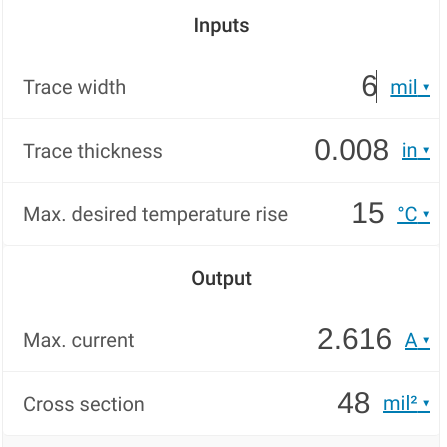
\includegraphics[scale=0.4]{figures/6_c}
		\caption{6mil Trace (1 inch length) }
	\end{minipage}
	\
	% Second image
	\begin{minipage}[b]{0.45\linewidth}
		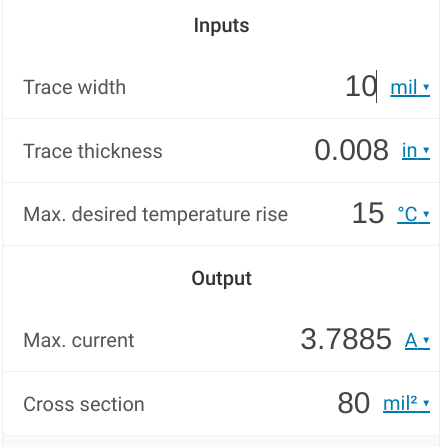
\includegraphics[scale=0.4]{figures/10_c}
		\caption{10mil Trace (1 inch length) }
	\end{minipage}
	\end{figure}\hspace{1cm}
	
	
	\begin{figure}[H]
	\centering
	\begin{minipage}[b]{0.45\linewidth}
		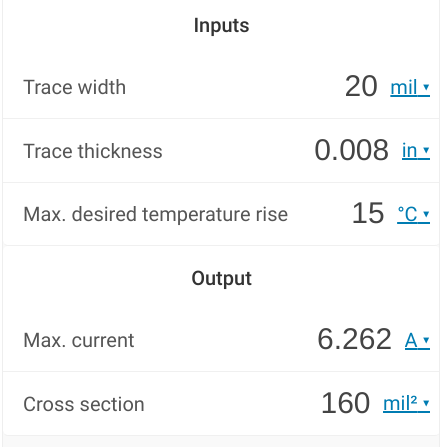
\includegraphics[scale=0.4]{figures/20_c}
		\caption{20mil Trace (1 inch length) }
	\end{minipage}
	\
	\begin{minipage}[b]{0.45\linewidth}
		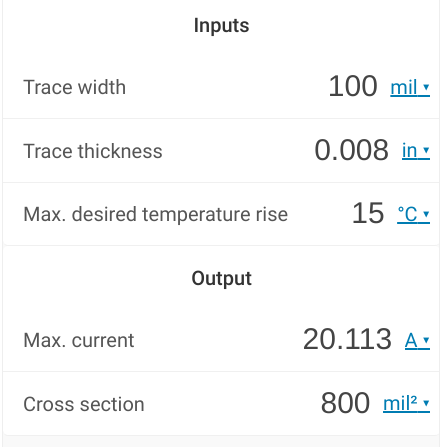
\includegraphics[scale=0.4]{figures/100_c}
		\caption{100mil Trace (1 inch length) }
	\end{minipage}
	\end{figure}

	Current when,
\begin{table}[H]
	\centering 
	\begin{tabular}{| l | c | c | c | c |}
		\hline
		\textbf{Trace witdth}&\textbf{Trace is Warm}&\textbf{Trace is Hot}&\textbf{Trace is Smoking}&\textbf{ $I_{max}$ Theoretical}\\\hline
		&&&&\\
\textbf{6 mils}&1.6A&2.3A&4.7A&2.616A\\
\textbf{10 mils}&2.4A&4A&6.5A&3.7885A\\
\textbf{20 mils}&3A&5.5A&10.3A&6.262A\\
\textbf{100 mils}&7.6A&10.3A&-&20.113A\\


\hline\hline
	\end{tabular}
	\caption{Observation and Readings for Max current}

\end{table}

This shows that we can run more current than expected theoretical values, we can run 1A of current easily on 6mils wide trace without making it warm.

\section{Learnings and Observation}\

\textbf{Problems with the 2-Wire Method}
\begin{enumerate}
	\item \textbf{Accuracy Issues:} The 2-wire method can give wrong readings because it counts the wire's resistance as part of what it's measuring. This is a big problem when measuring very low resistances.
	\item \textbf{Simple but Limited:} The 2-wire method is easy but not accurate for small resistances. This means it's not suitable for all situations.
\end{enumerate}

\textbf{Benefits of the 4-Wire (Kelvin) Method}
\begin{enumerate}
	\item \textbf{Better Accuracy:} The 4-wire method uses two sets of wires, one for the current and one for the voltage, which avoids the issue of counting the wire's resistance. This makes it much better for measuring low resistances accurately.
	\item \textbf{Accurate Readings:} It gives a true measure of an object's resistance without the extra resistance from the wires.
	
\end{enumerate}

\textbf{Important Practical Points}
\begin{enumerate}
	\item \textbf{Correct Use is Key:} Using the 4-wire method the right way is important. Wrong connections can lead to mistakes.
	\item 
	\textbf{Practice Helps Understanding:} Doing these experiments helps understand the theory better and shows how important it is to be precise and careful.
\end{enumerate}
	


\textbf{Current Capacity of Wires}
\begin{enumerate}
	\item \textbf{Heat and Wire Width:} The experiments showed that the width of a wire affects how much current it can carry without getting too hot. This is important for designing circuits that don't get damaged by heat.
	\item \textbf{Applying This Knowledge:} Learning the maximum current that different wire widths can carry helps in designing safer and more efficient circuits.
\end{enumerate}


\textbf{Specific Findings on Wire Current Capacity}
\begin{itemize}
	\item Wires that are 6mils wide can carry 1.6A.
	\item Wires that are 10mils wide can carry 2.4A.
	\item Wires that are 20mils wide can carry 3A.
	\item Wires that are 100mils wide can carry 7.6A.
\end{itemize}

These specific findings help in choosing the right wire width for different circuit needs.

\section{Conclusion}

The experiments have taught us more about how to measure resistance accurately and how wire width affects current capacity. We learned that the 2-wire method is not very accurate for low resistances, while the 4-wire method improves accuracy significantly. Also, understanding how much current a wire can carry without overheating helps in designing better circuits. This report shows the value of combining theory with practical experiments to improve electrical engineering designs.\\[10cm]


\hrule






%---------------------------------------------------------------------------
\end{document}
-
